\chapter{K-means clustering}
K-means clustering is an unsupervised machine learning algorithm for finding sub populations in unlabelled data.
It has not been applied to this case, but is reviewed for sake of completeness and to help understanding of Gaussian Mixture Models (See chapter \ref{sec:GMM}) 
\section{Theory} 

K-means basically works by iteratively estimating K cluster means and assigning responsibility according to euclidean distance.

\subsection{The K-means algorithm}
\begin{enumerate}

\item
Choose the number, K, of clusters to fit.

\item
Pick K random guesses of mean values $ \mu_j $ or mean vector $ \bm{\mu}_k $ for multi dimensional data.

\item \label{itm:Kmean_Est}
Assign responsibility of all data point by smallest euclidean distance to cluster mean.

\begin{equation}
r_{nk} =
  \begin{cases}
    1 & \text{if } k = 
    	\argmin_j \lVert \mathbf{x}_n - \bm{\mu}_j \rVert^2\\
    0 & \text{otherwise}
  \end{cases} 
\end{equation}

Where $ r_{nk} $ is 1 if cluster $ k $ is responsible for $ \mathbf{x}_n $ 

\item \label{itm:Kmean_Max}
Estimate new cluster means from cluster assignments

\begin{equation}
\bm{\mu}_k = 
\dfrac{\sum_n r_{nk}\mathbf{x}_n}
{\sum_n r_{nk}}
\end{equation}

\item
Repeat from \ref{itm:Kmean_Est}. until stopping criteria is met e.g. no change in cluster assignments or change in cluster means below pre-set threshold. 

\end{enumerate}
\textbf{}
\begin{figure}[H]
	\centering
	\begin{subfigure}[H]{0.3\linewidth}
		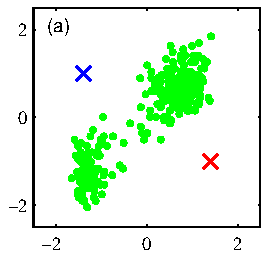
\includegraphics{Figure9_1a}
		\label{fig:F9.1a}
	\end{subfigure}
	\quad
	\begin{subfigure}[H]{0.3\linewidth}
		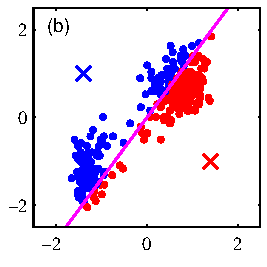
\includegraphics{Figure9_1b}
		\label{fig:F9.1b}
	\end{subfigure}
	\quad
	\begin{subfigure}[H]{0.3\linewidth}
		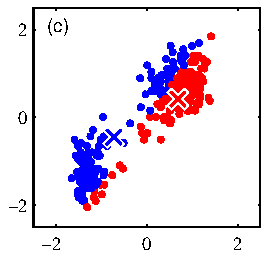
\includegraphics{Figure9_1c}
		\label{fig:F9.1c}
	\end{subfigure}
	
	
	\begin{subfigure}[H]{0.3\linewidth}
		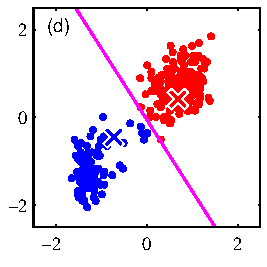
\includegraphics{Figure9_1d}
		\label{fig:F9.1d}
	\end{subfigure}
	\quad
	\begin{subfigure}[H]{0.3\linewidth}
		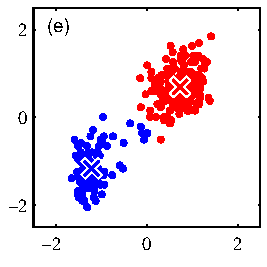
\includegraphics{Figure9_1e}
		\label{fig:F9.1e}
	\end{subfigure}
	\quad
	\begin{subfigure}[H]{0.3\linewidth}
		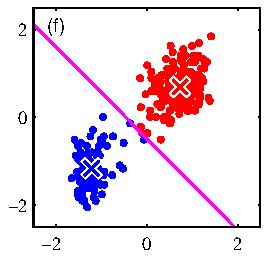
\includegraphics{Figure9_1f}
		\label{fig:F9.1f}
	\end{subfigure}
	

	\begin{subfigure}[H]{0.3\linewidth}
		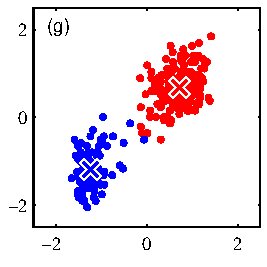
\includegraphics{Figure9_1g}
		\label{fig:F9.1g}
	\end{subfigure}
	\quad
	\begin{subfigure}[H]{0.3\linewidth}
		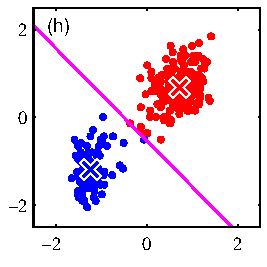
\includegraphics{Figure9_1h}
		\label{fig:F9.1h}
	\end{subfigure}
	\quad
	\begin{subfigure}[H]{0.3\linewidth}
		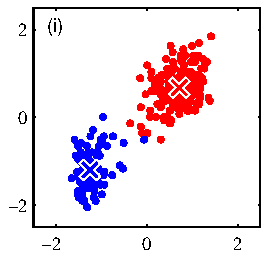
\includegraphics{Figure9_1i}
		\label{fig:F9.1i}
	\end{subfigure}
	
	\caption{Four iterations of K-means on the Old Faithful data set}

\end{figure}

In project like this K-means could used to make a sort of mixture model of each speaker, by fitting a number of clusters to the different unique sounds the individual speaker makes and then for a series of samples evaluating which speaker is most likely to have emitted the sounds.
  